\noindent
{\Large A-2. Random Generators}
\addcontentsline{toc}{section}{A-2. Random Generators}

\vspace*{7mm}

\noindent
In this section, I will explain how to generate random numbers. I
prepared five sample programs for the Cauchy distribution, Log Normal
distribution, Normal distribution, Uniform distribution and
Weibull distribution. 

\vspace*{20mm}

\noindent
{\Large A-2-1. Sample Program 6 (Cauchy)}
\addcontentsline{toc}{subsection}{A-2-1. Sample Program 6}
\index{Cauchy}

\vspace*{7mm}

\noindent
The equation for the Cauchy distribution is as follows.

\begin{equation}
f(x) = \frac{1}{\pi} \cdot \frac{1}{1+x^2}
\end{equation}

\noindent
The next program is a sample for the Cauchy distribution.

\vspace*{10mm}

{\footnotesize
\begin{center}
\begin{tabular}{|l|}\hline
\#include "Population.h"\\
\#include $<$fstream.h$>$\\
\#include $<$stdio.h$>$\\
\hspace*{\textwidth}\\
void main(void)\\
\{\\
\hspace*{10mm}// declaration\\
\hspace*{10mm}int seed      = 1234;\\
\hspace*{10mm}int i,j;\\
\hspace*{10mm}int total     = 1000000;\\
\hspace*{10mm}double r;\\
\hspace*{10mm}double rstore[total];\\
\hspace*{10mm}double start  = -50.05;\\
\hspace*{10mm}double end    =  50.05;\\
\hspace*{10mm}int div       =   1001;\\
\hspace*{10mm}double step   = (end-start)/div;\\
\hspace*{10mm}int counter[div];\\
\hspace*{10mm}double position[div];\\\hline
\end{tabular}
\vspace*{5mm}

{\small
Example 6. Sample Program 6-1.
}
\end{center}
}

\clearpage

{\footnotesize
\begin{center}
\begin{tabular}{|l|}\hline
\hspace*{10mm}// initialization\\
\hspace*{10mm}for (i=0;i$<$div;i++)\{\\
\hspace*{20mm}counter[i]=0;\\
\hspace*{10mm}\}\\
\\
\hspace*{10mm}// file open\\
\hspace*{10mm}FILE *fp;\\
\hspace*{10mm}fp = fopen("data.txt","w");\\
\\
\hspace*{10mm}// random seed\\
\hspace*{10mm}Rng::seed(seed);\\
\\
\hspace*{10mm}// random generator\\
\hspace*{10mm}for (i=0;i$<$total;i++)\{\\
\hspace*{20mm}r = Rng::cauchy();\\
\hspace*{20mm}rstore[i]=r;\\
\hspace*{20mm}for (j=0;j$<$div;j++)\{\\
\hspace*{30mm}position[j] = start + (j+j+1)*step/2.0;\\
\hspace*{30mm}if (r$>$=start+j*step \&\& r$<$start+(j+1)*step)\{\\
\hspace*{40mm}++counter[j];\\
\hspace*{30mm}\}\\
\hspace*{20mm}\}\\
\hspace*{10mm}\}\\
\\
\hspace*{10mm}// output\\
\hspace*{10mm}double prob;\\
\hspace*{10mm}for (j=0;j$<$div;j++)\{\\
\hspace*{20mm}prob = static\_cast$<$double$>$(counter[j]) / static\_cast$<$double$>$(total)/step;\\
\hspace*{20mm}fprintf(fp,"\%f \%f $\backslash$n",position[j],prob);\\
\hspace*{10mm}\}\\
\hspace*{\textwidth}\\
\}\\\hline
\end{tabular}
\vspace*{5mm}

{\small
Example 6. Sample Program 6-2.
}
\end{center}
}

\vspace*{10mm}

\noindent
The result of this program is shown in the next figure.

\clearpage

\begin{center}
\rotatebox{-90}{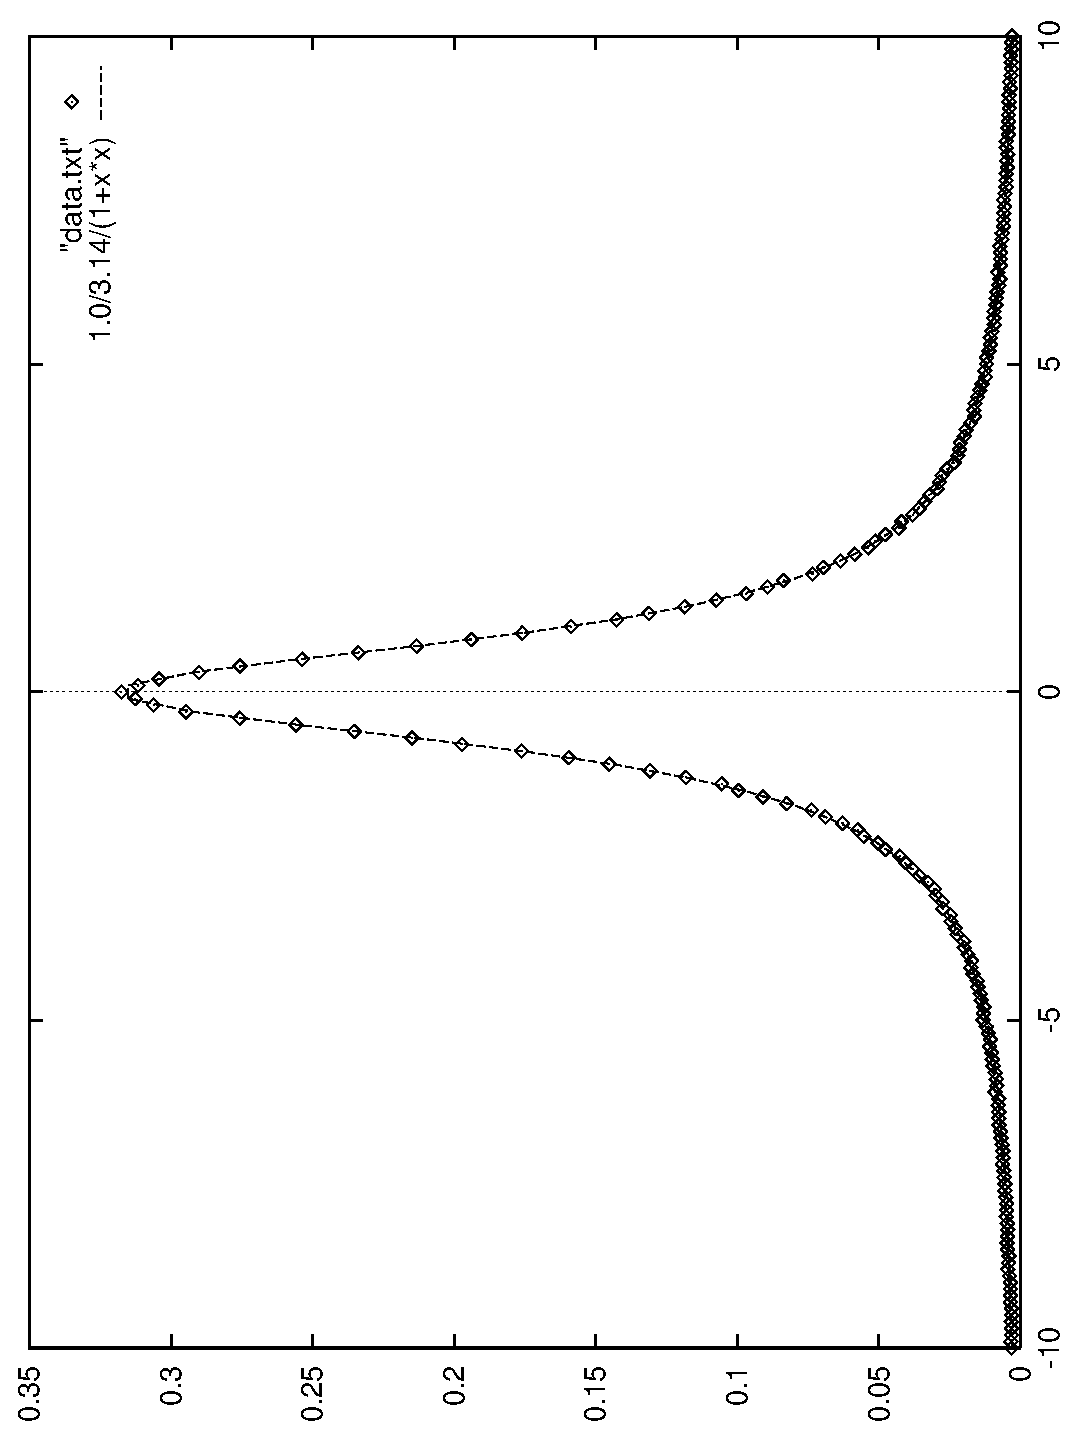
\includegraphics[height=12cm]{i-result-cauchy.eps}}\\
\vspace*{10mm}
Fig. A-2-1. The Cauchy distribution.\\
\end{center}

\vspace*{20mm}

\noindent
{\Large A-2-2. Sample Program 7 (Log Normal)}
\addcontentsline{toc}{subsection}{A-2-2. Sample Program 7}
\index{LogNormal}

\vspace*{7mm}

\noindent
The equation for the Log Normal distribution is as follows.

\begin{equation}
f(x) = \left\{
\begin{array}{ll}
\frac{1}{\sqrt{2\pi} \sigma x} \cdot \exp \left\{ \frac{-(\log x - \mu )^2}{2 \sigma^2} \right\} & x>0 \\
0 & x \le 0
\end{array}
\right.
\end{equation}

\noindent
Here,

\begin{equation}
\mu = \log \left( \frac{\mu_{log}^2}{\sqrt{\mu_{log}^2 +
\sigma_{log}^2}} \right)
\end{equation}

\begin{equation}
\sigma = \sqrt{\log \left( \frac{\mu_{log}^2+\sigma_{log}^2}{\mu_{log}^2} \right)}
\end{equation}

\noindent
In the program, I used 

\begin{equation}
\mu_{log} = \sqrt{e}
\end{equation}

\clearpage

\begin{equation}
\sigma_{log}^2 = e (e-1)
\end{equation}

\vspace*{5mm}

\noindent
The next program is a sample for the Log Normal distribution.

\vspace*{10mm}

{\footnotesize
\begin{center}
\begin{tabular}{|l|}\hline
\#include "Population.h"\\
\#include $<$fstream.h$>$\\
\#include $<$stdio.h$>$\\
\#include $<$LogNormal.h$>$\\
\hspace*{\textwidth}\\
void main(void)\\
\{\\
\\
\hspace*{10mm}// declaration\\
\hspace*{10mm}int seed      = 1234;\\
\hspace*{10mm}int i,j;\\
\hspace*{10mm}int total     = 1000000;\\
\hspace*{10mm}double r;\\
\hspace*{10mm}double rstore[total];\\
\hspace*{10mm}double start  = -0.005;\\
\hspace*{10mm}double end    = 10.005;\\
\hspace*{10mm}int div       =   1001;\\
\hspace*{10mm}double step   = (end-start)/div;\\
\hspace*{10mm}int counter[div];\\
\hspace*{10mm}double position[div];\\
\\
\hspace*{10mm}// instantialize\\
\hspace*{10mm}LogNormal lognormal;\\
\\
\hspace*{10mm}// initialization\\
\hspace*{10mm}for (i=0;i$<$div;i++)\{\\
\hspace*{20mm}counter[i]=0;\\
\hspace*{10mm}\}\\
\\
\hspace*{10mm}// file open\\
\hspace*{10mm}FILE *fp;\\
\hspace*{10mm}fp = fopen("data.txt","w");\\
\\
\hspace*{10mm}// random seed\\
\hspace*{10mm}Rng::seed(seed);\\\hline
\end{tabular}
\vspace*{5mm}

{\small
Example 7. Sample Program 7-1.
}
\end{center}
}

\clearpage

{\footnotesize
\begin{center}
\begin{tabular}{|l|}\hline
\hspace*{10mm}// random generator\\
\hspace*{10mm}for (i=0;i$<$total;i++)\{\\
\hspace*{20mm}lognormal.mean(SqrtE);\\
\hspace*{20mm}lognormal.variance(E*(E-1));\\
\hspace*{20mm}r = lognormal();\\
\hspace*{20mm}rstore[i]=r;\\
\hspace*{20mm}for (j=0;j$<$div;j++)\{\\
\hspace*{30mm}position[j] = start + (j+j+1)*step/2.0;\\
\hspace*{30mm}if (r$>$=start+j*step \&\& r<start+(j+1)*step)\{\\
\hspace*{40mm}++counter[j];\\
\hspace*{30mm}\}\\
\hspace*{20mm}\}\\
\hspace*{10mm}\}\\
\\
\hspace*{10mm}// output\\
\hspace*{10mm}double prob;\\
\hspace*{10mm}for (j=0;j$<$div;j++)\{\\
\hspace*{20mm}prob = static\_cast$<$double$>$(counter[j]) / static\_cast$<$double$>$(total)/step;\\
\hspace*{20mm}fprintf(fp,"\%f \%f $\backslash$n",position[j],prob);\\
\hspace*{10mm}\}\\
\hspace*{\textwidth}\\
\}\\\hline
\end{tabular}
\vspace*{5mm}

{\small
Example 7. Sample Program 7-2.
}
\end{center}
}

\vspace*{10mm}

\noindent
The result of this program is shown in the next figure.

\clearpage

\begin{center}
\rotatebox{-90}{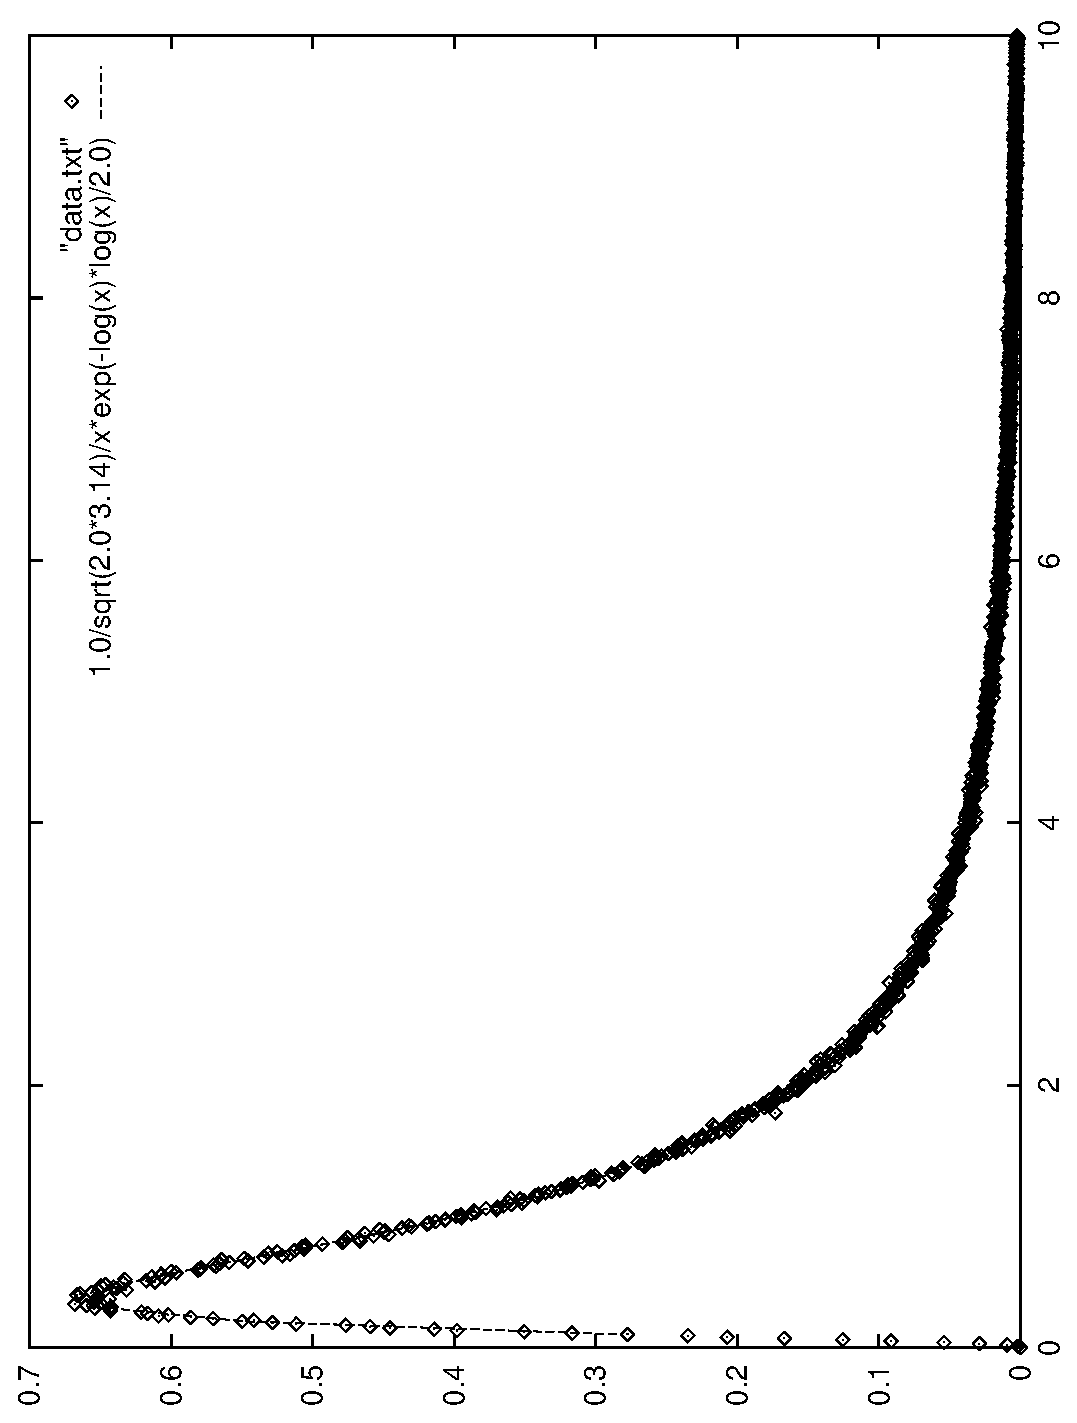
\includegraphics[height=12cm]{i-result-lognormal.eps}}\\
\vspace*{10mm}
Fig. A-2-2. The Log Normal distribution.\\
\end{center}

\vspace*{20mm}

\noindent
{\Large A-2-3. Sample Program 8 (Normal)}
\addcontentsline{toc}{subsection}{A-2-3. Sample Program 8}
\index{Normal}

\vspace*{7mm}

\noindent
The equation for the Normal distribution is as follows.

\begin{equation}
f(x) = \frac{1}{\sqrt{2\pi}\sigma} \cdot \exp{\frac{-(x-\mu)^2}{2\sigma^2}}
\end{equation}

\noindent
In the program, I used

\begin{equation}
\mu = 3 \hspace{3mm} , \hspace{3mm} \sigma^2 = 4
\end{equation}

\vspace*{5mm}

\noindent
The next program is a sample for the Normal distribution.

\clearpage

{\footnotesize
\begin{center}
\begin{tabular}{|l|}\hline
\#include "Population.h"\\
\#include $<$fstream.h$>$\\
\#include $<$stdio.h$>$\\
\hspace*{\textwidth}\\
void main(void)\\
\{\\
\\
\hspace*{10mm}// declaration\\
\hspace*{10mm}int seed      = 1234;\\
\hspace*{10mm}int i,j;\\
\hspace*{10mm}int total     = 1000000;\\
\hspace*{10mm}double r;\\
\hspace*{10mm}double rstore[total];\\
\hspace*{10mm}double start  = -3.006;\\
\hspace*{10mm}double end    =  9.006;\\
\hspace*{10mm}int div       =   1001;\\
\hspace*{10mm}double step   = (end-start)/div;\\
\hspace*{10mm}int counter[div];\\
\hspace*{10mm}double position[div];\\
\\
\hspace*{10mm}// initialization\\
\hspace*{10mm}for (i=0;i$<$div;i++)\{\\
\hspace*{20mm}counter[i]=0;\\
\hspace*{10mm}\}\\
\\
\hspace*{10mm}// file open\\
\hspace*{10mm}FILE *fp;\\
\hspace*{10mm}fp = fopen("data.txt","w");\\
\\
\hspace*{10mm}// random seed\\
\hspace*{10mm}Rng::seed(seed);\\
\\
\hspace*{10mm}// random generator\\
\hspace*{10mm}for (i=0;i$<$total;i++)\{\\
\hspace*{20mm}Rng::gauss.mean(3.0);\\
\hspace*{20mm}Rng::gauss.variance(4.0);\\
\hspace*{20mm}r = Rng::gauss();\\
\hspace*{20mm}rstore[i]=r;\\
\hspace*{20mm}for (j=0;j$<$div;j++)\{\\
\hspace*{30mm}position[j] = start + (j+j+1)*step/2.0;\\
\hspace*{30mm}if (r$>$=start+j*step \&\& r<start+(j+1)*step)\{\\
\hspace*{40mm}++counter[j];\\
\hspace*{30mm}\}\\
\hspace*{20mm}\}\\
\hspace*{10mm}\}\\\hline
\end{tabular}
\vspace*{5mm}

{\small
Example 8. Sample Program 8-1.
}
\end{center}
}

\clearpage

{\footnotesize
\begin{center}
\begin{tabular}{|l|}\hline
\hspace*{10mm}// output\\
\hspace*{10mm}double prob;\\
\hspace*{10mm}for (j=0;j$<$div;j++)\{\\
\hspace*{20mm}prob = static\_cast$<$double$>$(counter[j]) / static\_cast$<$double$>$(total)/step;\\
\hspace*{20mm}fprintf(fp,"\%f \%f $\backslash$n",position[j],prob);\\
\hspace*{10mm}\}\\
\hspace*{\textwidth}\\
\}\\\hline
\end{tabular}
\vspace*{5mm}

{\small
Example 8. Sample Program 8-2.
}
\end{center}
}

\vspace*{10mm}

\noindent
The result of this program is shown in the next figure.

\vspace*{10mm}

\begin{center}
\rotatebox{-90}{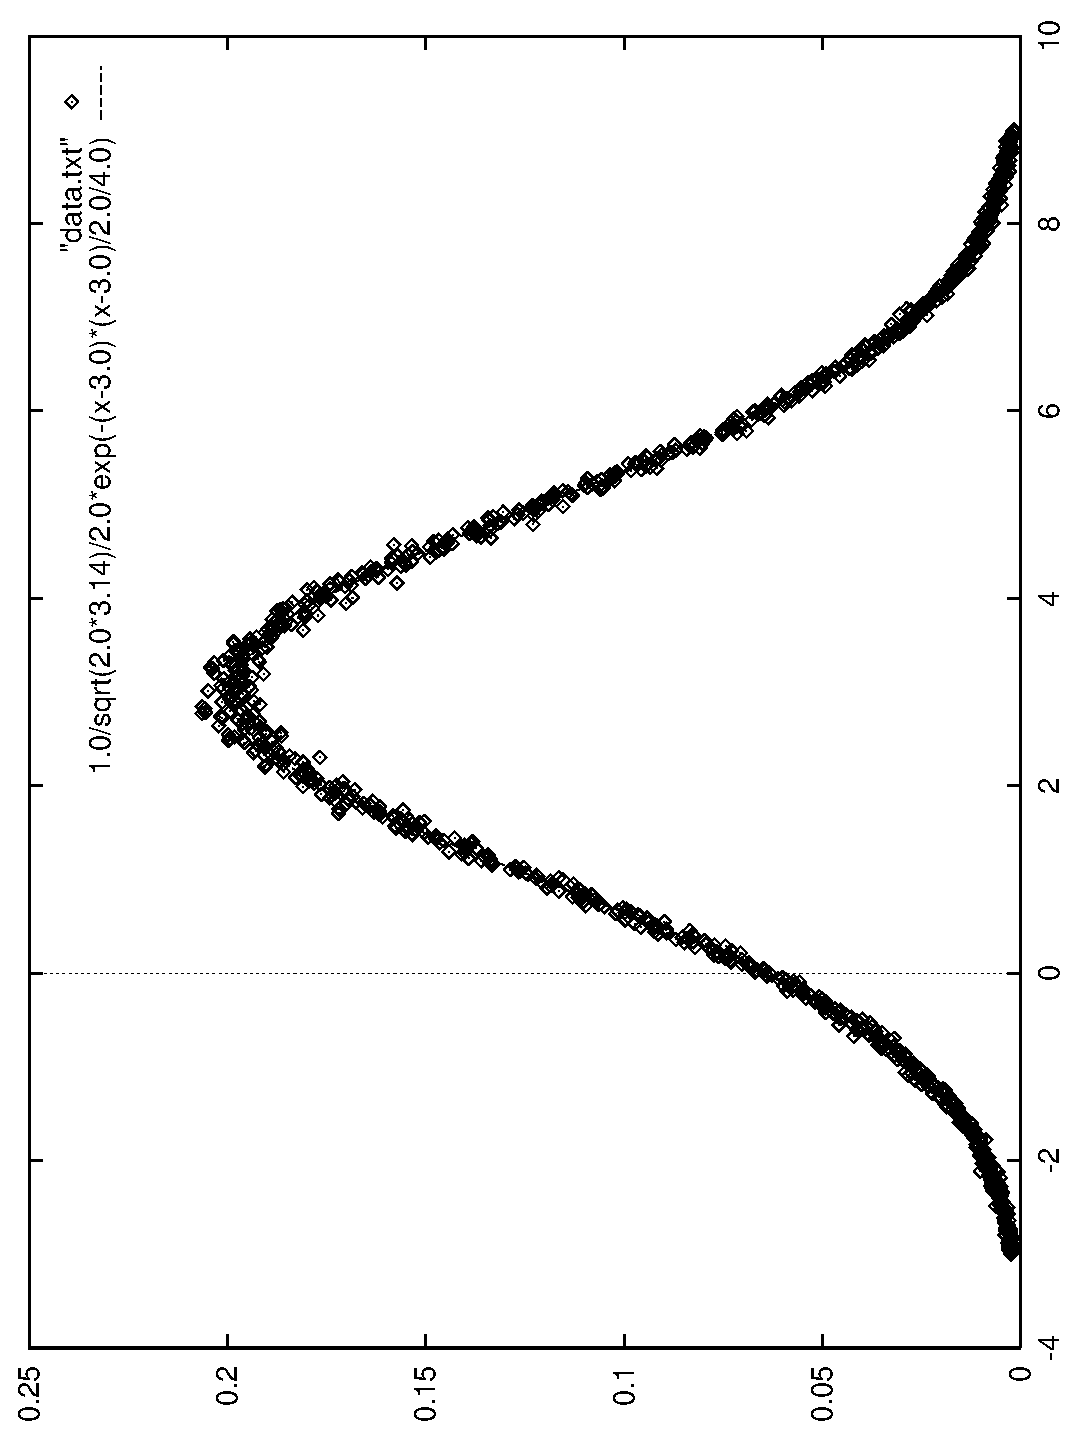
\includegraphics[height=12cm]{i-result-normal.eps}}\\
\vspace*{10mm}
Fig. A-2-3. The Normal distribution.\\
\end{center}

\clearpage

\noindent
{\Large A-2-4. Sample Program 9 (Uniform)}
\addcontentsline{toc}{subsection}{A-2-4. Sample Program 9}
\index{Uniform}

\vspace*{7mm}

\noindent
The equation for the Uniform distribution is as follows.

\begin{equation}
f(x) = \left\{
\begin{array}{ll}
1 / ( x_{upper} - x_{lower} )  & x_{lower} \le x \le x_{upper} \\
0 & the \hspace{2mm} other
\end{array}
\right.
\end{equation}

\noindent
In the program, I used

\begin{equation}
x_{lower} = 1.0 \hspace{3mm} , \hspace{3mm} x_{upper} = 2.0
\end{equation}

\vspace*{5mm}

\noindent
The next program is a sample for the Uniform distribution.

\vspace*{10mm}

{\footnotesize
\begin{center}
\begin{tabular}{|l|}\hline
\#include "Population.h"\\
\#include $<$fstream.h$>$\\
\#include $<$stdio.h$>$\\
\hspace*{\textwidth}\\
void main(void)\\
\{\\
\\
\hspace*{10mm}// declaration\\
\hspace*{10mm}int seed      = 1234;\\
\hspace*{10mm}int i,j;\\
\hspace*{10mm}int total     = 1000000;\\
\hspace*{10mm}double r;\\
\hspace*{10mm}double rstore[total];\\
\hspace*{10mm}double start  = 1.0;\\
\hspace*{10mm}double end    = 2.0;\\
\hspace*{10mm}int div       = 1000;\\
\hspace*{10mm}double step   = (end-start)/div;\\
\hspace*{10mm}int counter[div];\\
\hspace*{10mm}double position[div];\\
\\
\hspace*{10mm}// initialization\\
\hspace*{10mm}for (i=0;i$<$div;i++)\{\\
\hspace*{20mm}counter[i]=0;\\
\hspace*{10mm}\}\\\hline
\end{tabular}
\vspace*{5mm}

{\small
Example 9. Sample Program 9-1.
}
\end{center}
}  

\clearpage

{\footnotesize
\begin{center}
\begin{tabular}{|l|}\hline
\hspace*{10mm}// file open\\
\hspace*{10mm}FILE *fp;\\
\hspace*{10mm}fp = fopen("data.txt","w");\\
\\
\hspace*{10mm}// random seed\\
\hspace*{10mm}Rng::seed(seed);\\
\\
\hspace*{10mm}// random generator\\
\hspace*{10mm}for (i=0;i$<$total;i++)\{\\
\hspace*{20mm}Rng::uni.low(start);\\
\hspace*{20mm}Rng::uni.high(end);\\
\hspace*{20mm}r = Rng::uni();\\
\hspace*{20mm}rstore[i]=r;\\
\hspace*{20mm}for (j=0;j$<$div;j++)\{\\
\hspace*{30mm}position[j] = start + (j+j+1)*step/2.0;\\
\hspace*{30mm}if (r$>$=start+j*step \&\& r<start+(j+1)*step)\{\\
\hspace*{40mm}++counter[j];\\
\hspace*{30mm}\}\\
\hspace*{20mm}\}\\
\hspace*{10mm}\}\\
\\
\hspace*{10mm}// output\\
\hspace*{10mm}double prob;\\
\hspace*{10mm}for (j=0;j$<$div;j++)\{\\
\hspace*{20mm}prob = static\_cast$<$double$>$(counter[j]) / static\_cast$<$double$>$(total)/step;\\
\hspace*{20mm}fprintf(fp,"\%f \%f $\backslash$n",position[j],prob);\\
\hspace*{10mm}\}\\
\\
\}\\\hline
\end{tabular}
\vspace*{5mm}

{\small
Example 9. Sample Program 9-2.
}
\end{center}
}  

\vspace*{5mm}

\noindent
The result of this program is shown in the next figure.

\clearpage

\begin{center}
\rotatebox{-90}{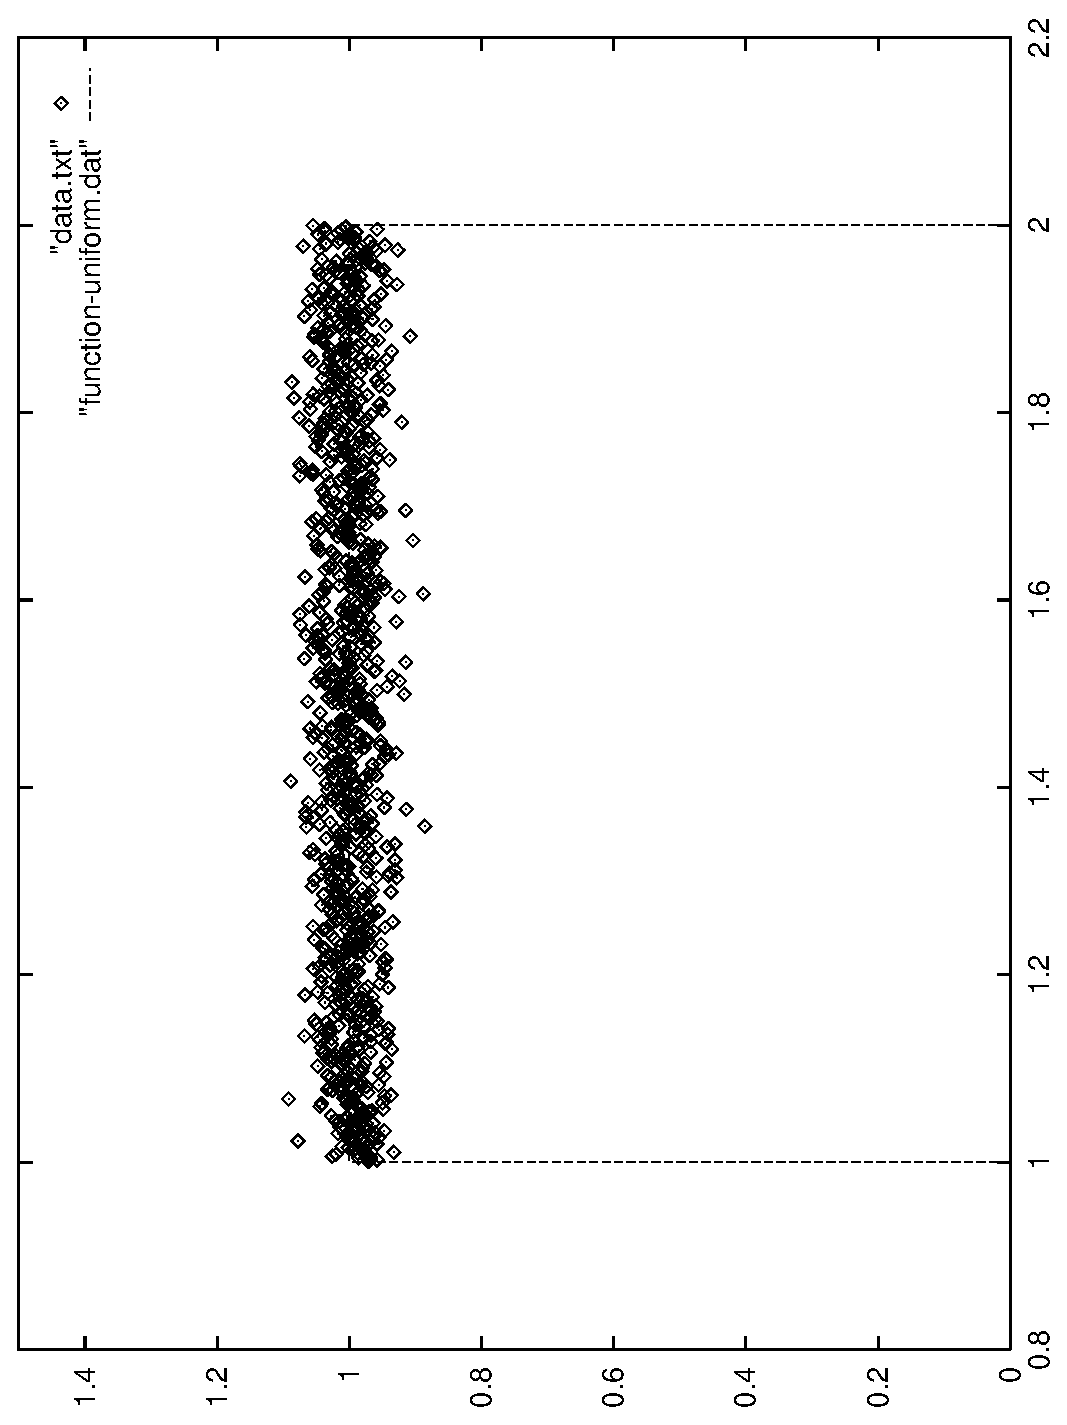
\includegraphics[height=12cm]{i-result-uniform.eps}}\\
\vspace*{10mm}
Fig. A-2-4. The Uniform distribution.\\
\end{center}

\vspace*{20mm}

\noindent
{\Large A-2-5. Sample Program 10 (Weibull)}
\addcontentsline{toc}{subsection}{A-2-5. Sample Program 10}
\index{Weibull}

\vspace*{7mm}

\noindent
The equation for the Weibull distribution is as follows.

\begin{equation}
f(x) = \frac{\alpha}{\beta} \cdot \exp \left\{ - \frac{1}{\beta} x^\alpha \right\} \cdot x^{\alpha-1}
\end{equation}

\noindent
In the program, I used

\begin{equation}
\alpha = 2  \hspace{3mm} , \hspace{3mm} \beta = 3
\end{equation}

\vspace*{5mm}

\noindent
The next program is a sample for the Weibull distribution.

\clearpage

{\footnotesize
\begin{center}
\begin{tabular}{|l|}\hline
\#include "Population.h"\\
\#include $<$fstream.h$>$\\
\#include $<$stdio.h$>$\\
\#include $<$Weibull.h$>$\\
\hspace*{\textwidth}\\
void main(void)\\
\{\\
\\
\hspace*{10mm}// declaration\\
\hspace*{10mm}int seed      = 1234;\\
\hspace*{10mm}int i,j;\\
\hspace*{10mm}int total     = 1000000;\\
\hspace*{10mm}double r;\\
\hspace*{10mm}double rstore[total];\\
\hspace*{10mm}double start  = -0.005;\\
\hspace*{10mm}double end    = 10.005;\\
\hspace*{10mm}int div       = 1001;\\
\hspace*{10mm}double step   = (end-start)/div;\\
\hspace*{10mm}int counter[div];\\
\hspace*{10mm}double position[div];\\
\\
\hspace*{10mm}// instantialize\\
\hspace*{10mm}Weibull weibull;\\
\\
\hspace*{10mm}// initialization\\
\hspace*{10mm}for (i=0;i$<$div;i++)\{\\
\hspace*{20mm}counter[i]=0;\\
\hspace*{10mm}\}\\
\\
\hspace*{10mm}// file open\\
\hspace*{10mm}FILE *fp;\\
\hspace*{10mm}fp = fopen("data.txt","w");\\
\\
\hspace*{10mm}// random seed\\
\hspace*{10mm}Rng::seed(seed);\\
\hspace*{10mm}// random generator\\
\hspace*{10mm}for (i=0;i$<$total;i++)\{\\
\hspace*{20mm}weibull.alpha(2.0);\\
\hspace*{20mm}weibull.beta(3.0);\\
\hspace*{20mm}r = weibull();\\
\hspace*{20mm}rstore[i]=r;\\
\hspace*{20mm}for (j=0;j$<$div;j++)\{\\
\hspace*{30mm}position[j] = start + (j+j+1)*step/2.0;\\
\hspace*{30mm}if (r$>$=start+j*step \&\& r$<$start+(j+1)*step)\{\\
\hspace*{40mm}++counter[j];\\\hline
\end{tabular}
\vspace*{5mm}

{\small
Example 10. Sample Program 10-1.
}
\end{center}
}  

\clearpage

  
{\footnotesize
\begin{center}
\begin{tabular}{|l|}\hline

\hspace*{30mm}\}\\
\hspace*{20mm}\}\\
\hspace*{10mm}\}\\
\\
\hspace*{10mm}// output\\
\hspace*{10mm}double prob;\\
\hspace*{10mm}for (j=0;j$<$div;j++)\{\\
\hspace*{20mm}prob = static\_cast$<$double$>$(counter[j]) / static\_cast$<$double$>$(total)/step;\\
\hspace*{20mm}fprintf(fp,"\%f \%f $\backslash$n",position[j],prob);\\
\hspace*{10mm}\}\\
\hspace*{\textwidth}\\
\}\\\hline
\end{tabular}
\vspace*{5mm}

{\small
Example 10. Sample Program 10-2.
}
\end{center}
}  
  
\vspace*{5mm}

\noindent
The result of this program is shown in the next figure.

\vspace*{5mm}

\begin{center}
\rotatebox{-90}{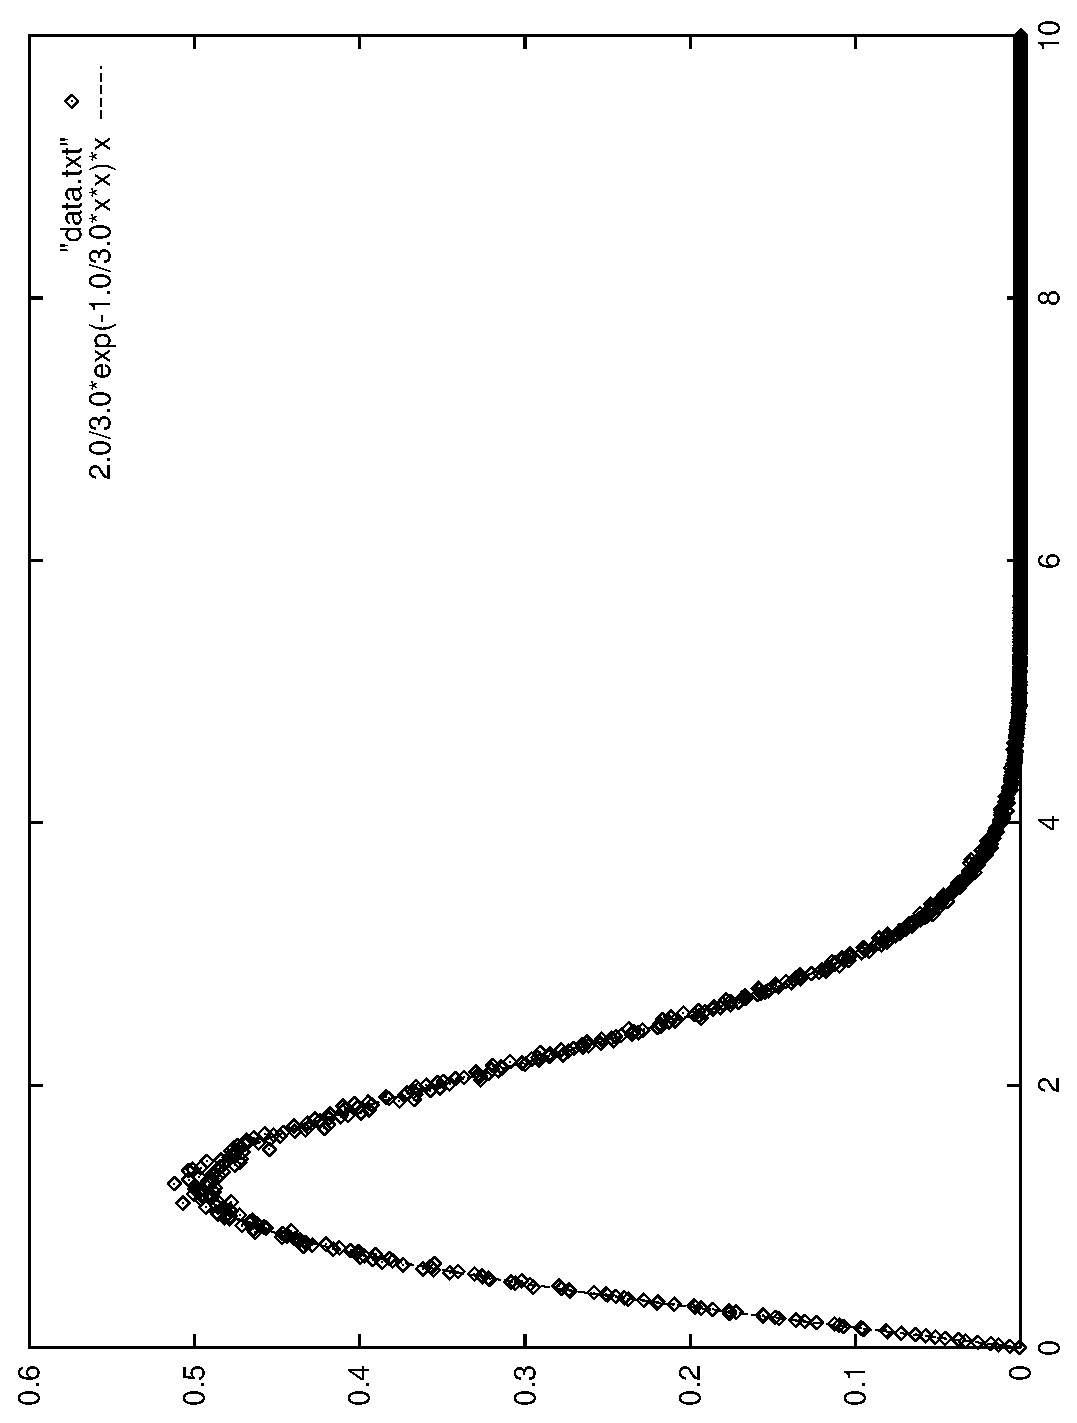
\includegraphics[height=12cm]{i-result-weibull.eps}}\\
\vspace*{10mm}
Fig. A-2-5. Weibull distribution.\\
\end{center}





